\documentclass[12pt,a4paper,titlepage]{book}
\usepackage{graphicx} 
\author{Kacper Zieliński}
\title{Rybki}
\date{10 styczeń 2020} 
\begin{document}
\maketitle
\tableofcontents
\newpage
\begin{enumerate}
\item Karpiowate
\begin{itemize}
\item Karp
\item Karaś
\item Płotka
\end{itemize}
\item Okoniowate
\begin{itemize}
\item Okoń
\item Sandacz
\end{itemize}
\item Łososiowate
\begin{itemize}
\item Łosoś
\item Pstrag
\item Troć
\end{itemize}
\end{enumerate}

\chapter{Karpiowate}
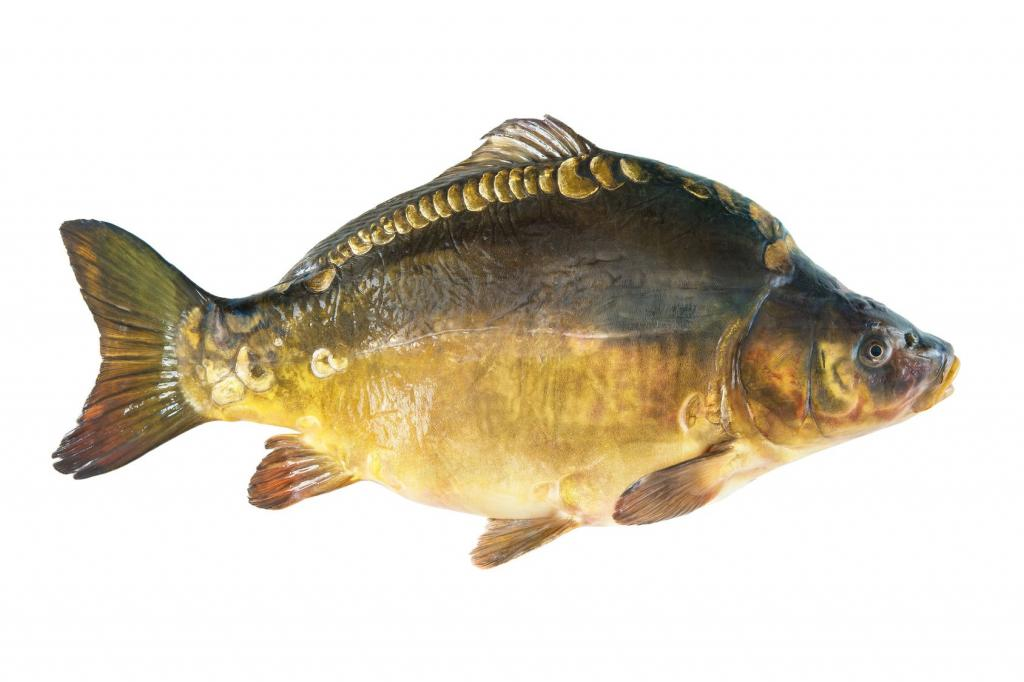
\includegraphics[width=50mm,height=!]{karp}
\section{Karp}
Zlewiska mórz Czarnego, Kaspijskiego i Aralskiego. Liczne odmiany hodowlane sa rozpowszechnione zarówno w hodowli, jak i w wodach otwartych na całym niemal świecie.
\section{Karaś}
Preferuje małe i płytkie zbiorniki wodne. W Polsce jest spotykany we wszystkich nizinnych wodach śródladowych, stojacych i wolno płynacych, w miejscach o porośnietym roślinami podłożu.
\section{Płoć}
Wystepuje w całej Europie z wyjatkiem Półwyspu Iberyjskiego, zlewiska Adriatyku, Grecji oraz północnej Skandynawii, na wschodzie siega daleko w głab Azji. Wystepuje we wszystkich wodach słodkich w Polsce także w wodach przybrzeżnych Bałtyku.
\begin{table}
\begin{center}
\begin{tabular}{|c||l|l|}
\hline Najwieksza & długość & waga \\ \hline \hline
Karp & 107,0 cm & 34,50 kg  \\
Karaś & 48,5 cm & 4,160 kg  \\
Płoć & 47,0 cm & 1,57 kg  \\ \hline
\end{tabular}
\end{center}
\end{table}
\chapter{Okoniowate}
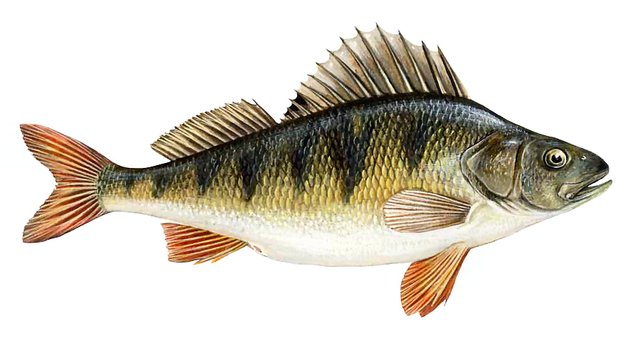
\includegraphics[width=50mm,height=!]{okon}
\section{Okoń}
Wystepuje w wodach do 1000 m n.p.m., zarówno w płynacych jak i stojacych a także w słonawych wodach przybrzeżnych w estuarium rzek. Młodsze osobniki czesto tworza ławice, starsze żyja w niewielkich grupach badź samotnie.
\section{Sandacz}
Wystepuje w jeziorach, zbiornikach zaporowych, średnich i dużych nizinnych rzekach, wyrobiskach oraz w płytkich wodach przybrzeżnych Bałtyku. Preferuje głebokie, metne wody o twardym, piaszczystym, żwirowatym badź gliniastym dnie. Jest wrażliwy na niedobór tlenu.
\begin{table}
\begin{center}
\begin{tabular}{|c||l|l|}
\hline Najwieksza & długość & waga \\ \hline \hline
Okoń & 50,0 cm & 2,69 kg  \\
Sandacz & 108,0 cm & 14,20 kg  \\ \hline
\end{tabular}
\end{center}
\end{table}
\chapter{Łososiowate}
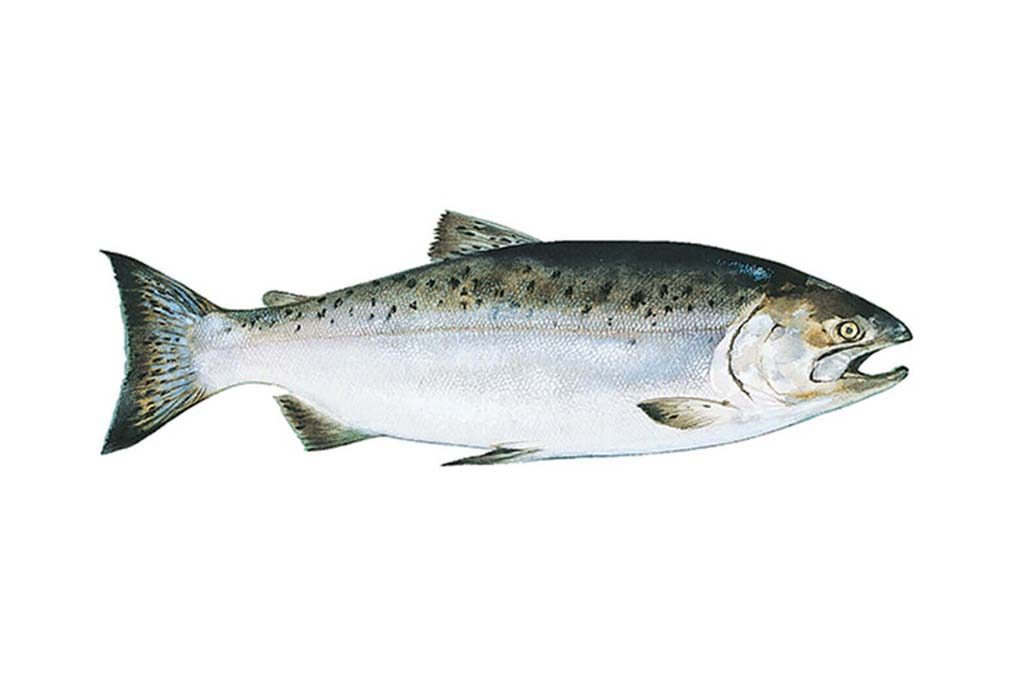
\includegraphics[width=50mm,height=!]{losos}
\section{Łosoś}
W północnej cześci Atlantyku, w rzekach Ameryki Północnej, w Europie od Portugalii po Morze Białe, Północne i Bałtyk. W jeziorach Ładoga i Onega tworzy formy wyłacznie słodkowodne.
\section{Pstrag}
W Polsce liczny na południu i północy kraju. Wystepuje w górskich potokach Beskidów, Tatr, Sudetów, Jury Krakowsko-Czestochowskiej, także w rzekach Dolnego Ślaska, Pomorza Zachodniego i Środkowego, na Warmii i Mazurach, w dopływach Warty.
\section{Troć}
Wody słodkie Europy i zachodniej Azji oraz przybrzeżne wody morskie wokół Europy i północno-zachodniej Afryki. Introdukowane w co najmniej 24 krajach, głównie w Europie i obydwu Amerykach, a także w kilku krajach Azji oraz w Australii.
\begin{table}

\begin{center}
\begin{tabular}{|c||l|l|}
\hline Najwieksza & długość & waga \\ \hline \hline
Łosoś & 130,0 cm & 30,40 kg  \\
Pstrag & 77,5 cm & 5,526 kg  \\
Troć & 105,0 cm & 14,60 kg  \\ \hline
\end{tabular}
\end{center}
\end{table}
\chapter{Równania}
\begin{equation}
2+2=4
\end{equation}
$$\lim_{n \to \infty} \frac{n}{12}=\infty$$
$$f(x)= \frac{ \frac{z^5+3z^3}{z+3} }
{ \frac{\log(z)}{z+3}*\frac{z^3+3z}{z-3}}$$

\begin{thebibliography}{9}
\bibitem{lamport94}
 Kacper Zielński,
 \emph{Rybki}.
 1 wydanie, Gdańsk
 2020.
\end{thebibliography}

\end{document}
